\documentclass[12pt]{article}
\usepackage[english]{babel}
\usepackage{natbib}
\usepackage{url}
\usepackage[utf8x]{inputenc}
\usepackage{amsmath}
\usepackage{graphicx}
\usepackage{hyperref}
\graphicspath{{images/}}
\usepackage{parskip}
\usepackage{fancyhdr}
\usepackage{vmargin}
\setmarginsrb{3 cm}{2.5 cm}{3 cm}{2.5 cm}{1 cm}{1.5 cm}{1 cm}{1.5 cm}
\usepackage{hyperref}

\title{BeerEX: the Beer EXpert system}
\author{Donato Meoli}
\date{September 11, 2019}

\makeatletter
\let\thetitle\@title
\let\theauthor\@author
\let\thedate\@date
\makeatother

\pagestyle{fancy}
\fancyhf{}
\rhead{\theauthor}
\lhead{\thetitle}
\cfoot{\thepage}

\begin{document}

\begin{titlepage}
	\centering
    \vspace*{0.5 cm}
    
\includegraphics[scale = 0.5]{img/unipi.png}\\[1.0 cm]
    \textsc{\LARGE University of Pisa}\\[0.5 cm]
    \textsc{\Large Department of Computer Science}\\[1.5 cm]
	\textsc{\large Artificial Intelligence Fundamentals}\\[0.5 cm]
	\rule{\linewidth}{0.2 mm} \\[0.4 cm]
	{ \huge \bfseries \thetitle}\\
	\rule{\linewidth}{0.2 mm} \\[1.5 cm]
	\centering \textsc{\large \emph{Author:}}\\[0.5 cm]
	\begin{minipage}{0.4\textwidth}
		\begin{center} \large
			\textbf{\theauthor}
		\end{center}
		\end{minipage}~
		\begin{minipage}{0.4\textwidth}
	\end{minipage}\\[2 cm]
	{\large \thedate}\\[2 cm]
	\vfill
\end{titlepage}

\tableofcontents
\pagebreak

\section{Context \& Background}

\subsection{The Context of BeerEX}
The expert system \textit{BeerEX} (Beer EXpert system) was designed to suggest a beer to drink according to taste and meal. The choice of building such a system was dictated by the vastness of the product market and by the lack of information that is usually found in consumers. The system is essentially useful for people who want to taste appropriate beers and would like to know in real time the most suitable beer based on their tastes and/or based on the meals they are going to consume. Through simple questions the system recognizes the tastes of the user returning also indications on how each question helps to arrive at the solution of the problem. BeerEX works with a dataset of beer styles, therefore a limited domain on which the rules have greater inferential power, thus not providing for recommending any beer on the market, but rather the style to which it is associated. Each style of beer has characteristics about the \textit{flavor}, \textit{color}, \textit{alcohol} content and \textit{carbonation}, etc.: all aspects on which the user will be able to express their preferences. The system uses the dataset made available by the American association \href{https://www.craftbeer.com}{CraftBeer}. \\At the beginning of 2016, in the United States alone, there are more than 5,000 breweries responsible for the various beer brands, around 150 different beer styles and over 20,000 brands. Furthermore, the market is expanding more and more: according to the estimates of the \href{https://www.brewersassociation.org}{Brewers Association} there was an increase of about 800 breweries compared to the previous year (always in the US market), for a total of 129,000 employees in the sector and an economic impact of around 56 billion dollars.

\begin{figure}[h]
\centering
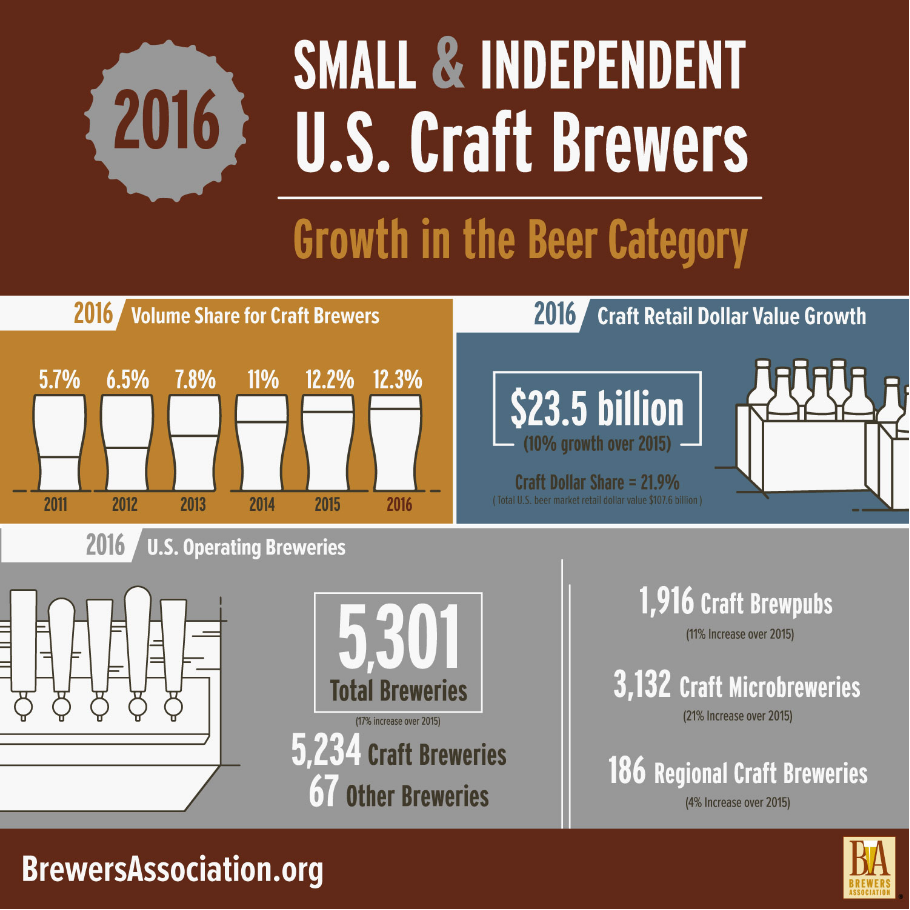
\includegraphics[scale = 0.4]{img/brewers.png}
\caption{Operative breweries in the United States in 2016}
\end{figure}

\subsection{Why an Expert System}
Conventional programming languages ​​are designed for procedural data manipulation. Humans, however, often solve complex problems using very abstract symbolic approaches that cannot be implemented with conventional languages. One of the research results in the area of ​​Artificial Intelligence has been the development of techniques that allow the modeling of information at higher levels of abstraction. These techniques are incorporated into logical languages ​​or tools that allows to build programs that closely resemble human logic in their implementation and are therefore easier to develop and maintain. Some of these tools, which emulate human skills in well-defined problem domains, are called expert systems. Rules based programming is one of the most commonly used techniques for developing expert systems. In this programming paradigm, rules and facts are used to represent the knowldge and then, the inference engine, with a powerful pattern matching algorithm, called Rete, will verify the matching of a rule through his left-hand side (LHS) in accordance with the state of the world or the working memory.

\begin{figure}[h]
\centering
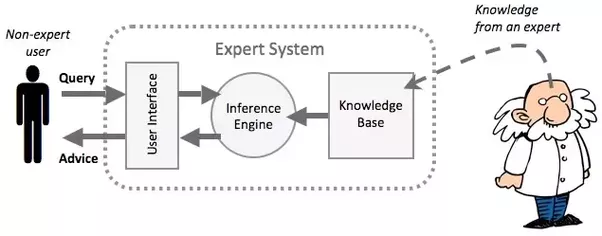
\includegraphics[scale = 0.6]{img/arch.png}
\caption{Architecture of an Expert System.}
\end{figure}


\subsection{CLIPS: a Tool for building Expert Systems}
\textit{CLIPS} - \textit{C Language Integrated Production System} - is a tool for building rule-based expert systems.
I suoi aspetti chiave sono:

\begin{itemize}
\item rappresentazione della Conoscenza;
\item portabilità;
\item integrazione/estensibilità;
\item sviluppo interattivo.
\end{itemize}

\begin{figure}[h]
\centering
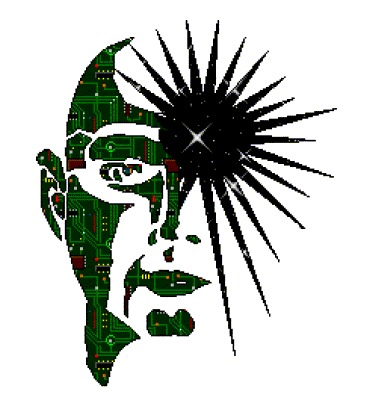
\includegraphics[scale = 0.16]{img/clips.jpg}
\caption{CLIPS logo.}
\end{figure}


\section{System Analysis}

\subsection{Use Cases}
Il sistema è in grado di riconoscere lo \textbf{scenario d’utenza}, tramite alcune domande iniziali più generiche inerenti il \textbf{sesso}, la fascia d’\textbf{età}, la \textbf{stagione} attuale, la \textbf{frequenza} con cui l’utente è solito bere birra, se dovrà bere birra e \textbf{fumare} al contempo:
\begin{itemize}
\item \textbf{Sesso}: il sesso dell’utente è utile, seppur in bassa misura, per determinare quanto forte in termini di alcool e gusto sarà la birra consigliata. \\Domanda associata: “Are you male or female?” \\Risposte valide: male, female;

	\item Fascia d’\textbf{età}: l’età dell’utente è utile per determinare quanto forte in termini di alcool e gusto sarà la birra consigliata. \\Domanda associata: “How old are you?” \\Risposte valide: 18-23, 24-29, $\geq30$;

\item \textbf{Stagione}: le condizioni meteorologiche influenzano le nostre percezioni e necessità. La scelta di una birra è tra questi. \\Domanda associata: “It is autumn, spring, summer or winter?” \\Risposte valide: autumn, spring, summer, winter;

\item \textbf{Frequenza}: la frequenza con cui l’utente è solito bere birra ci aiuta nel proporre birre più particolari nel caso in cui l’utente sia più avvezzo al bere birra e, quindi, sarà probabilmente più predisposto nell’accettare proposte di birre meno comuni. \\Domanda associata: “Are you a regular beer drinker?” \\Risposte valide: yes, no;

\item \textbf{Fumatore}: il sapore del tabacco potrebbe alterare il gusto della birra; inoltre, birre dal sapore molto intense potrebbero legare particolarmente bene con il gusto del tabacco. \\Domanda associata: “Are you going to smoke while you drink?” \\Risposte valide: yes, no.
\end{itemize}

Una volta avvenuto il primo riconoscimento, il sistema è in grado di adattare le sue conoscenze all’utente che ha di fronte. In questa maniera le domande poste ad un utente non saranno necessariamente le stesse poste ad un altro.

\subsection{Esecuzione}

Le domande che il sistema porrà dopo aver individuato lo scenario d'uso saranno relative a preferenze personali, come colore, gradazione alcolica, carbonatazione e sapore preferiti, tipo di pasto che l’utente si accinge a consumare, principale componente del pasto in questione e sua eventuale differenziazione, principale metodo di cottura del pasto.
\\Poste tali domande il sistema restituirà le birre più appropriate ritrovate sulla base delle risposte ricevute; sarà possibile, quindi, selezionando il link relativo, accedere alla pagina www.craftbeer.com per leggere la scheda dettagliata della birra in disamina.

\begin{figure}[h]
\centering
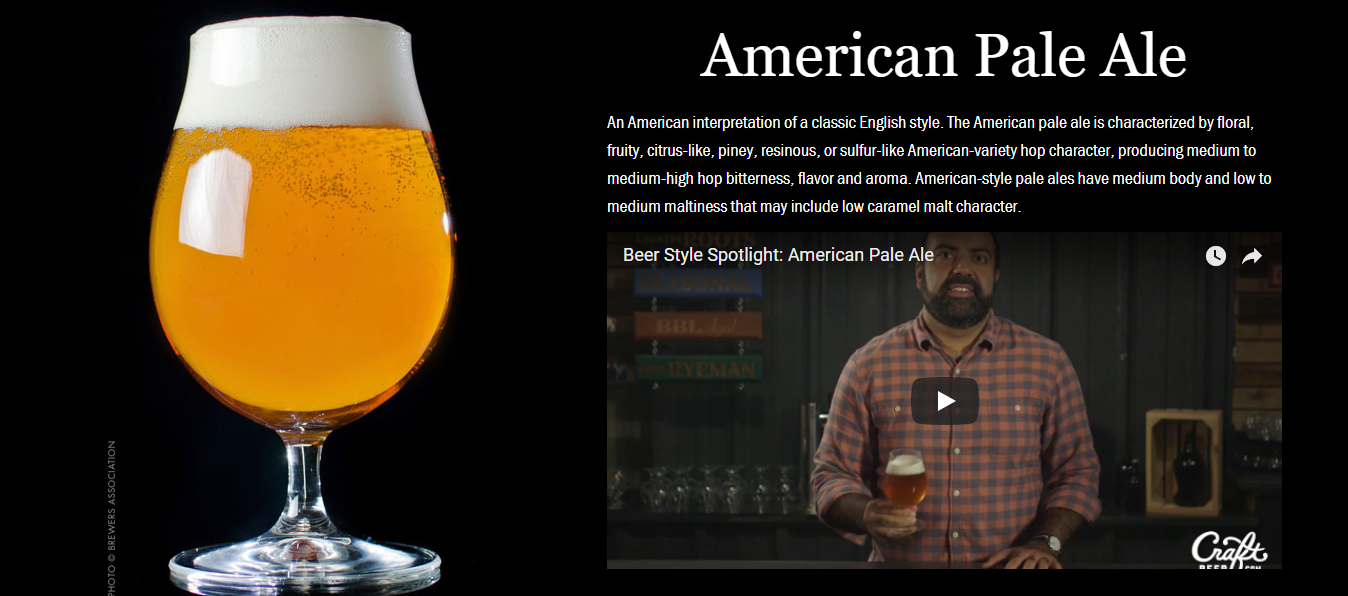
\includegraphics[width=15cm,height=8cm,keepaspectratio]{img/beer.png}
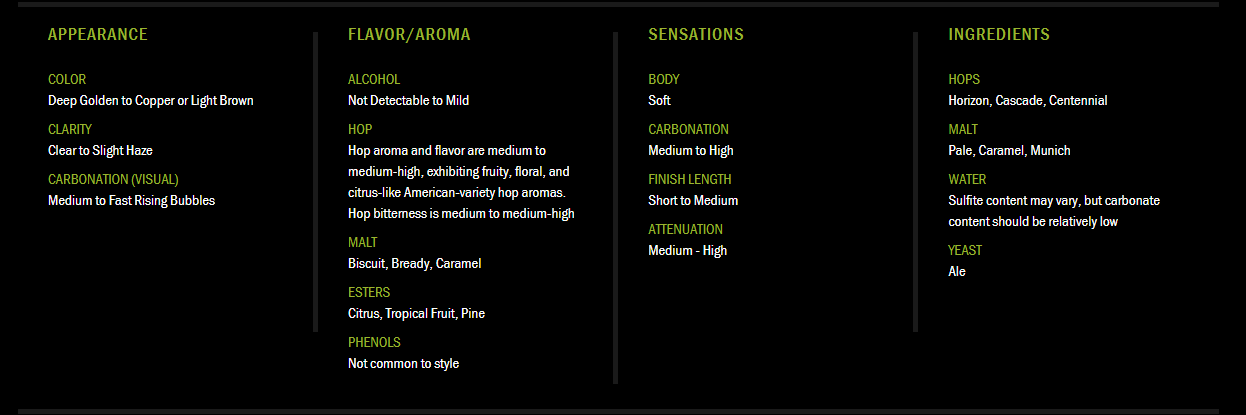
\includegraphics[width=15cm,height=8cm,keepaspectratio]{img/details.png}
\caption{Esempio della scheda della birra American Pale Ale, del sito Craftbeer.com.}
\end{figure}

\subsection{Use Aids}
Il sistema è adatto per più \textit{gradi di esperienza} dell’utente sul dominio birra ed è adatto per un qualsiasi range di età; è sottointeso che il sistema debba essere utilizzato da utenti maggiorenni e, quindi, abilitati per legge al consumo di alcool. Un eventuale utente in difficoltà di fronte al sistema avrà a disposizione, ove disponibili (sono state escluse domande banali), due possibili comandi:
\begin{itemize}
\item \textbf{help}: tale comando consentirà all’utente di mostrare un aiuto nella descrizione della domanda per una migliore comprensione della stessa;
\item \textbf{why}: tale comando consentirà all’utente di mostrare una motivazione del perchè la domanda è stata posta.
\end{itemize}

\begin{figure}[h]
\centering
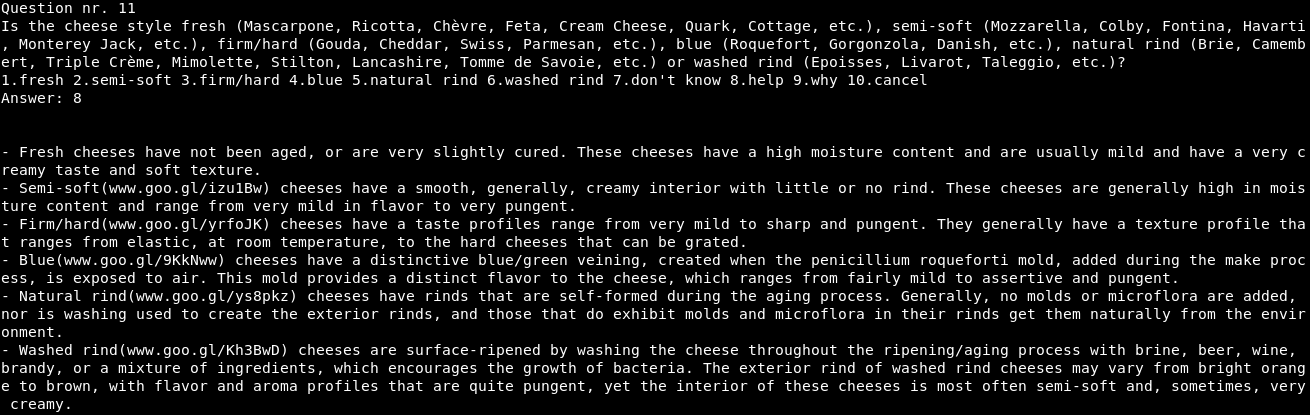
\includegraphics[width=15cm,height=9cm,keepaspectratio]{img/help.png}
\caption{Esempio di help.}
\end{figure}

\begin{figure}[h]
\centering
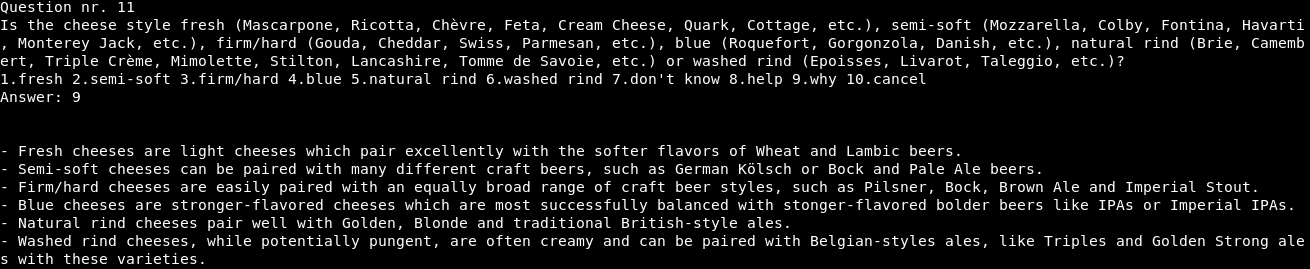
\includegraphics[width=15cm,height=9cm,keepaspectratio]{img/why.png}
\caption{Esempio di why.}
\end{figure}

\subsection{System Modules}

Il sistema è diviso in più file:
\begin{itemize}
\item \textbf{beerex.clp}: file contenente i template delle definizioni; richiama inoltre gli altri file contenenti domande, conoscenza e base di dati;
\item \textbf{beer-questions.clp}: file contenente tutte le domande;
\item \textbf{beer-knowledge.clp}: file contenente la conoscenza dell’esperto in relazione al dominio applicativo;
\item \textbf{beer-styles.fct}: racchiude la base di dati degli stili di birre.
\end{itemize}

\subsection{Reasoning under Uncertainty}

La conoscenza del sistema è incerta: in generale, nei sistemi esperti, si fa uso di una probabilità soggettiva formulata da esperti. Una teoria statistica dell'evidenza è fornita dalla statistica di Bayes che, essendo computazionalmente intrattabile è stata utilizzata per mettere a punto i \textit{fattori di certezza}, ossia dei meccanismi relativamente informali per quantificare i livelli di fiducia da assegnare a una determinata conclusione sulla base di fatti comprovati. In BeerEX è possibile che due o più regole possano trarre conclusioni su fatti asseriti nella working memory con diversi fattori di certezza. Al fine di calcolare il fattore di certezza BeerEX combina questi pesi usando la seguente formula per ottenere un singolo fattore di certezza:

\[
   CF(X,Y) =
   \begin{cases}
      X+Y-XY & se X,Y > 0 \\
      X+Y+XY & se X,Y < 0 \\
      \frac{X+Y}{1-min(|X|,|Y|)} & altrimenti
   \end{cases}
\]

dove X e Y sono i fattori di certezza compresi nell'intervallo [-1; 1], dove -1 indica il massimo grado di sfiducia con il quale si asserisce il fatto, 1 indica il massimo grado di fiducia con il quale si asserisce il fatto, mentre $\forall$ n $\in$ (-1; 1) si esprimono tutti i gradi di verità intermedi.

\subsection{Risultati e Ritrattazione}

Al termine dell'esecuzione vengono proposte le birre più adeguate e viene proposta una spiegazione delle scelte effettuate dal sistema. Vi è, inoltre, la possibilità di effettuare una ritrattazione: il sistema conserva nella working memory la lista delle domande alla quale si è risposto. Una funzione in CLIPS preleva questa lista e resetta la memoria fino alla domanda che l’utente vuole ritrattare e la ripropone. Facendo così viene cancellato tutto quello che si è asserito da quella domanda in poi. Se l’utente risponde negativamente alla richiesta da parte del sistema di ritrattare il programma termina l’esecuzione.

\newpage
\section{Extensions}

\subsection{Telegram ChatBot}
Come emerso dai test con gli utenti, uno dei problemi maggiormente evidenziati è stato la difficoltà di utilizzo del sistema, definita poco \textit{user-friendly} e, soprattutto, poco utile in quanto la reale utilità del sistema può sovvenire non davanti ad un computer, bensì durante le uscite quotidiane in pub e ristoranti.\\A questo proposito, essendo \textit{CLIPS} un tool portabile e embeddabile, è stato pensato di renderlo fruibile aldilà di un ambiente CLI, permettendogli di interagire per mezzo di un chatbot simulando una conversazione con l'esperto, lasciando inalterata la parte logica del sistema in linguaggio \textit{CLIPS}.

\begin{figure}[h]
\centering
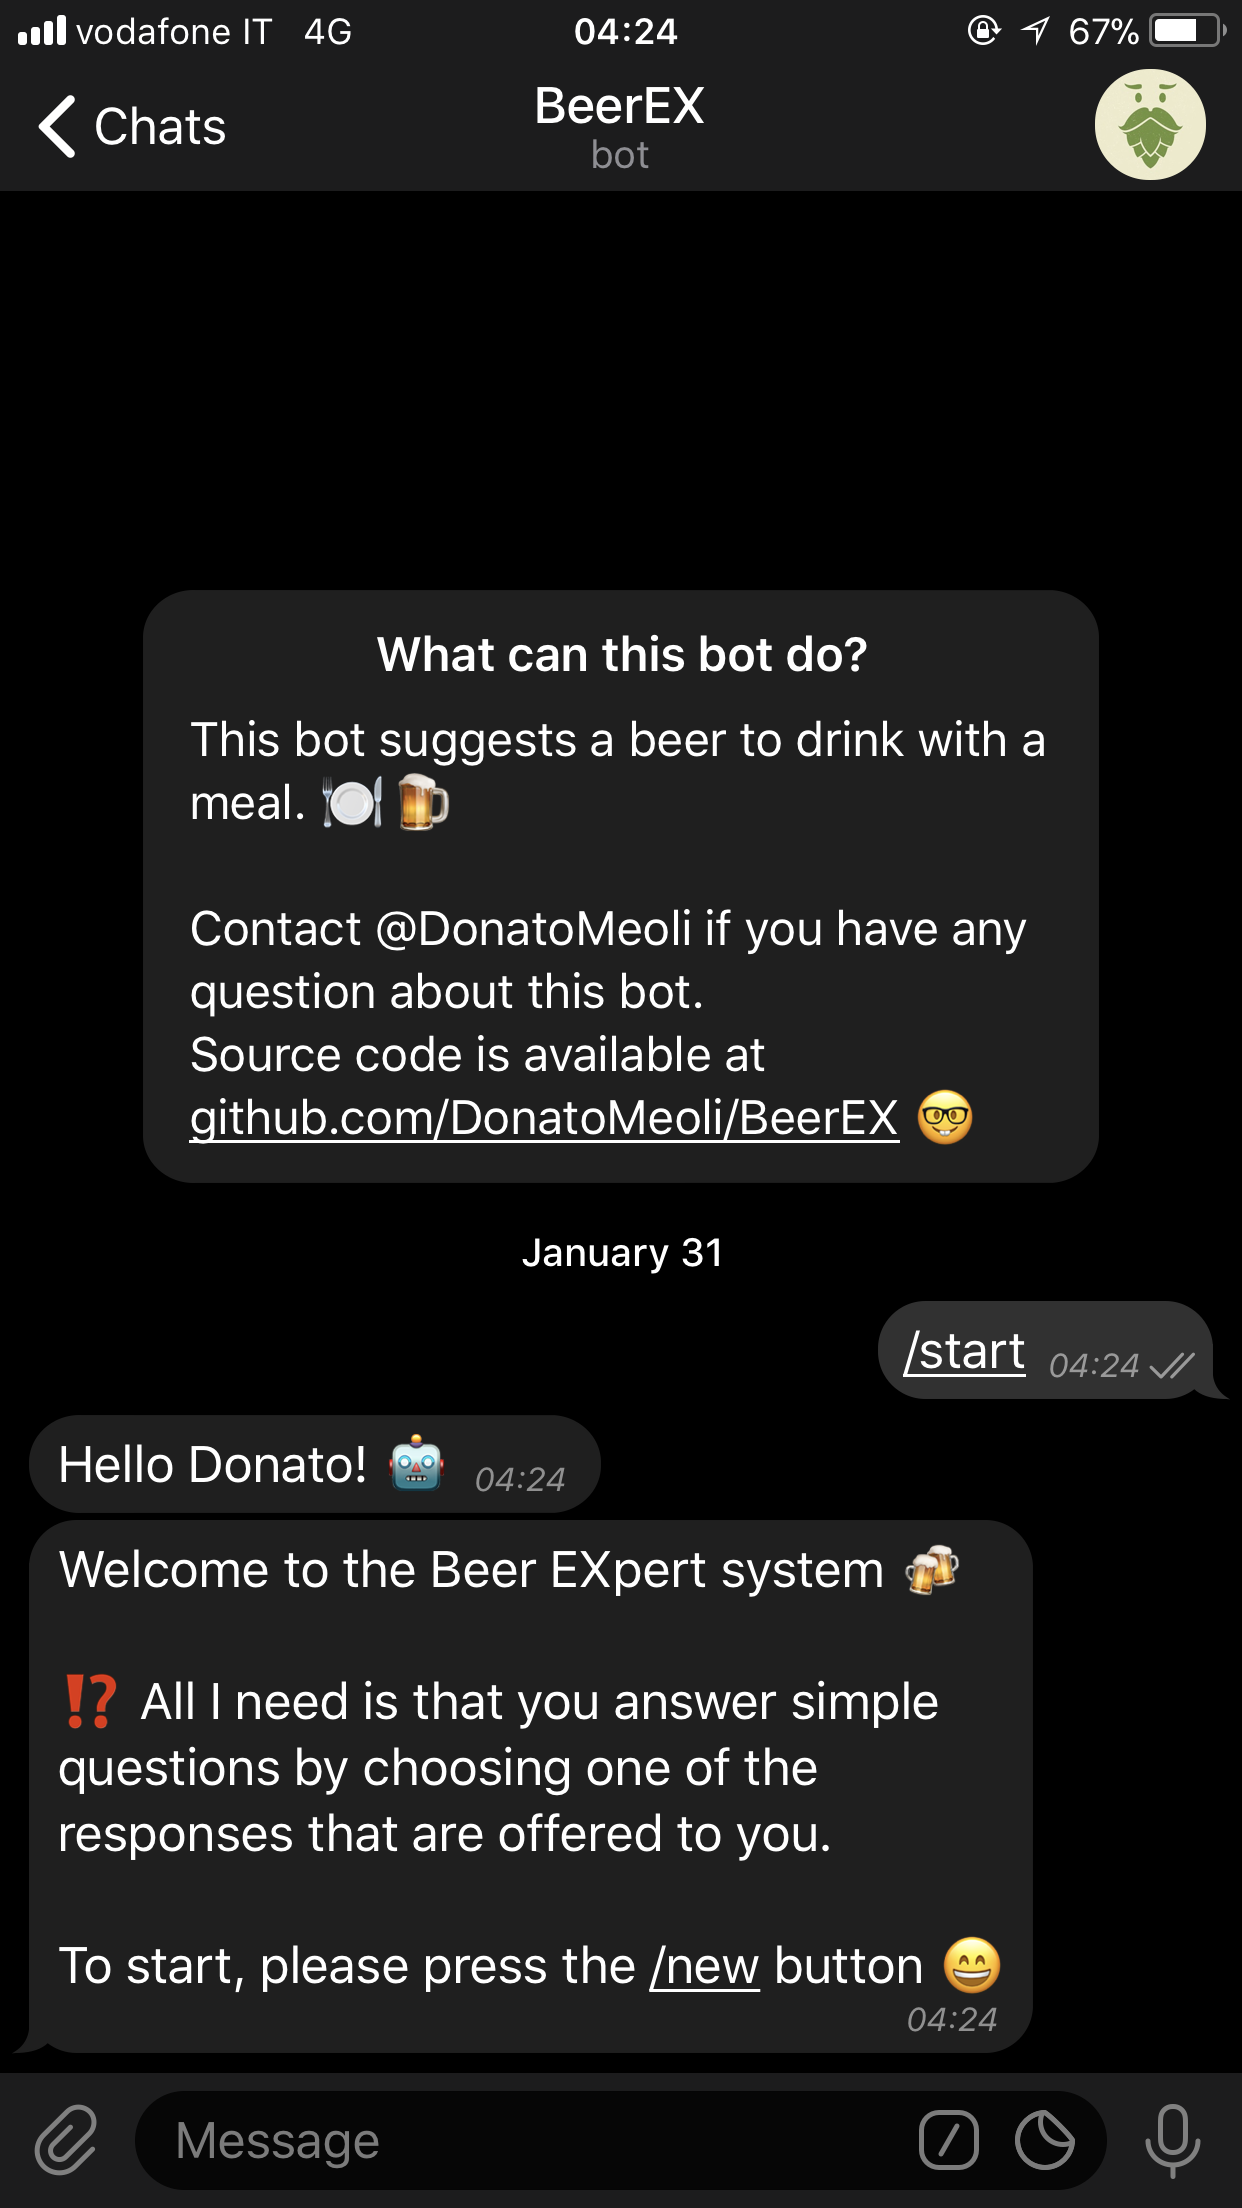
\includegraphics[scale=0.13]{img/bot1.png}\quad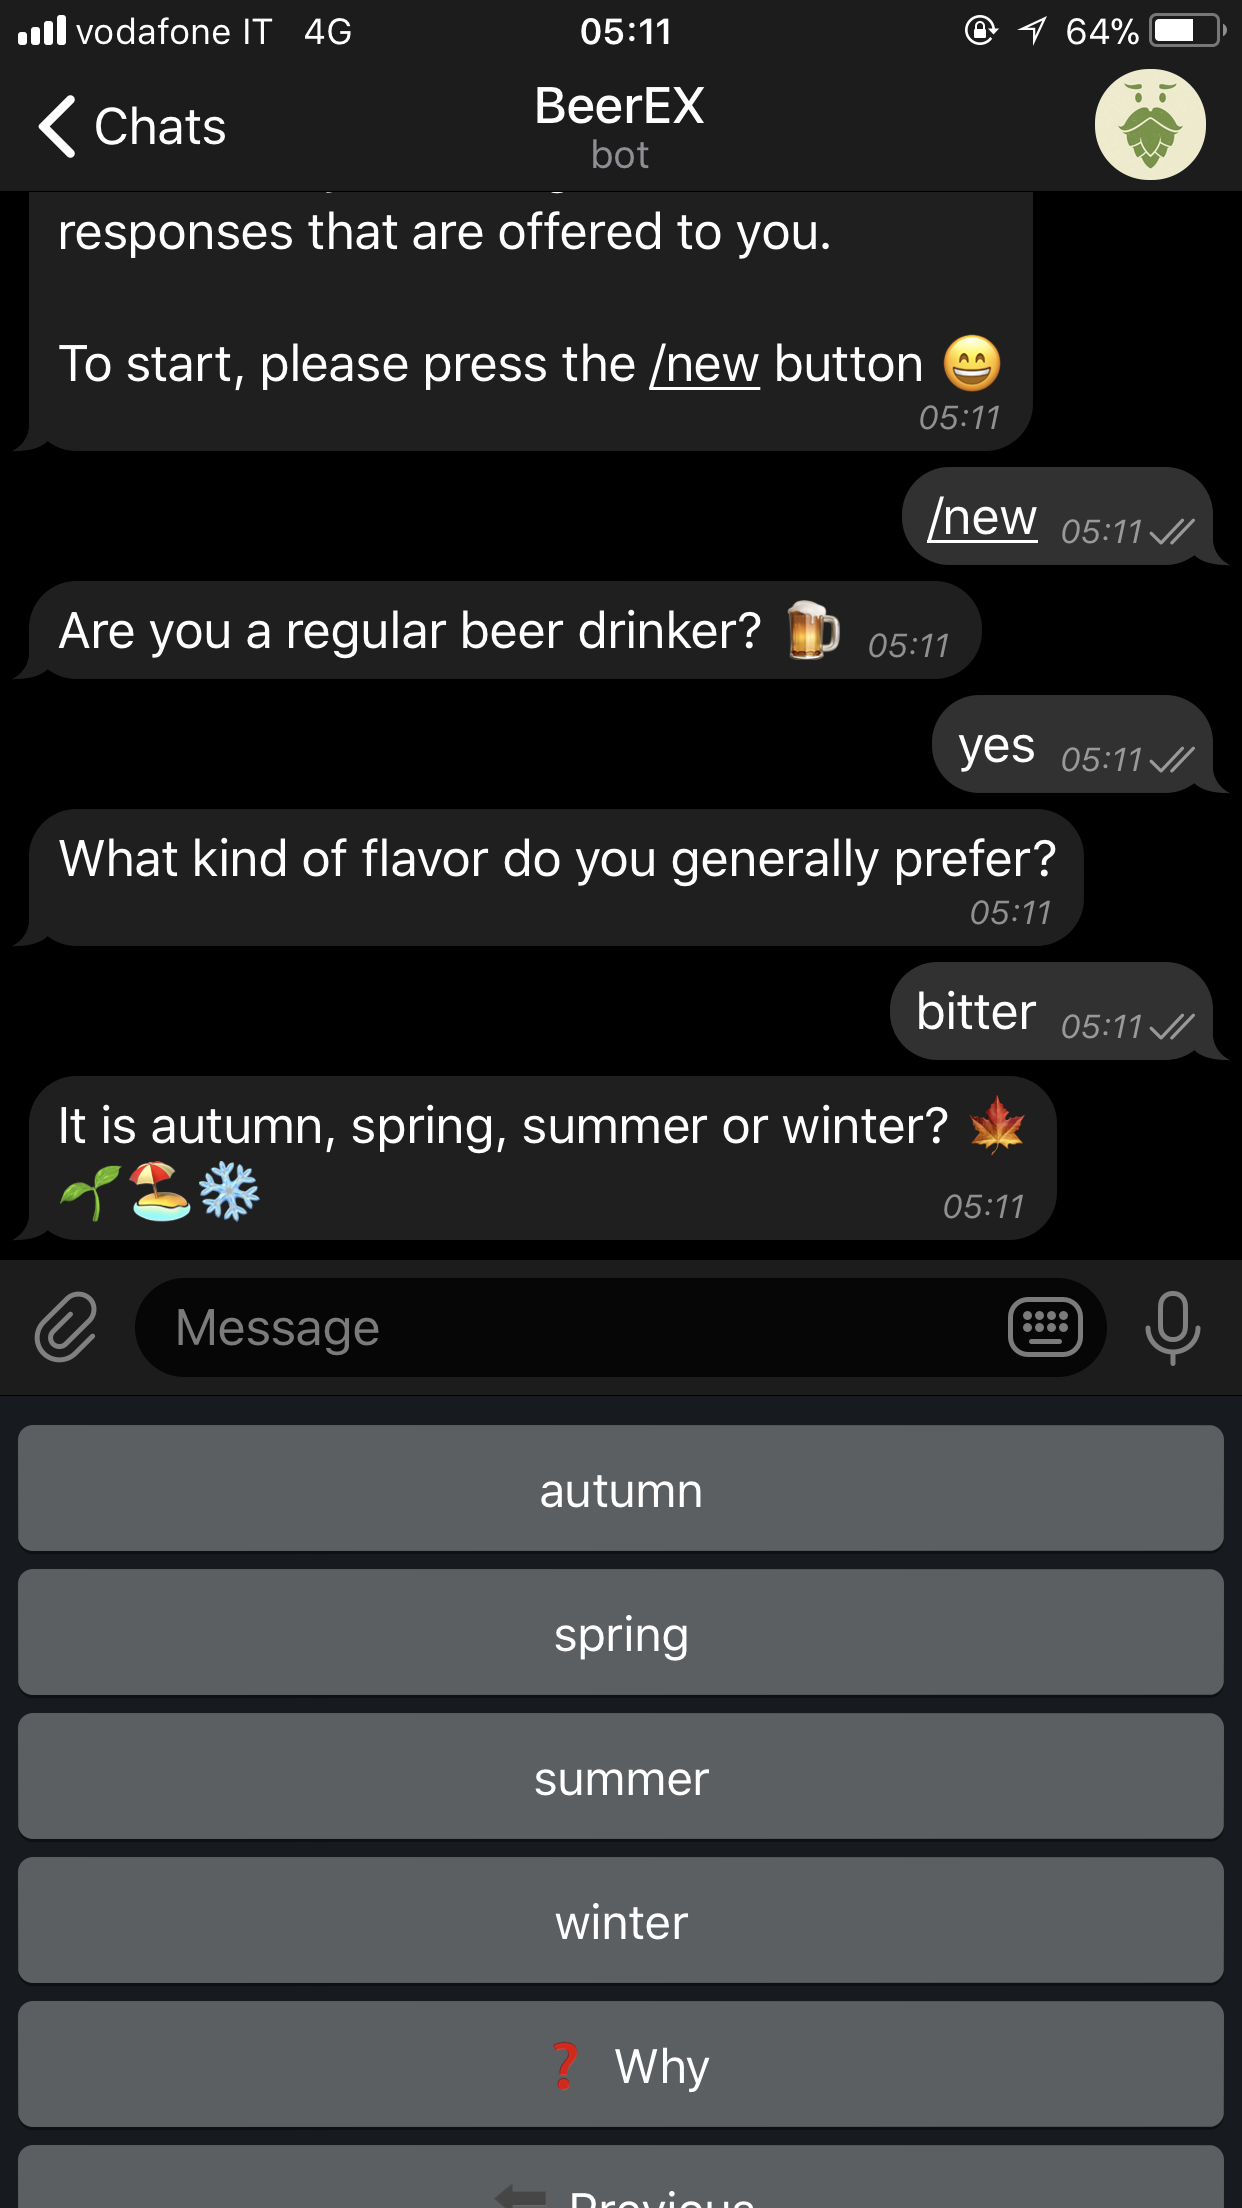
\includegraphics[scale=0.13]{img/bot2.png}
\end{figure}
\begin{figure}[h]
\centering
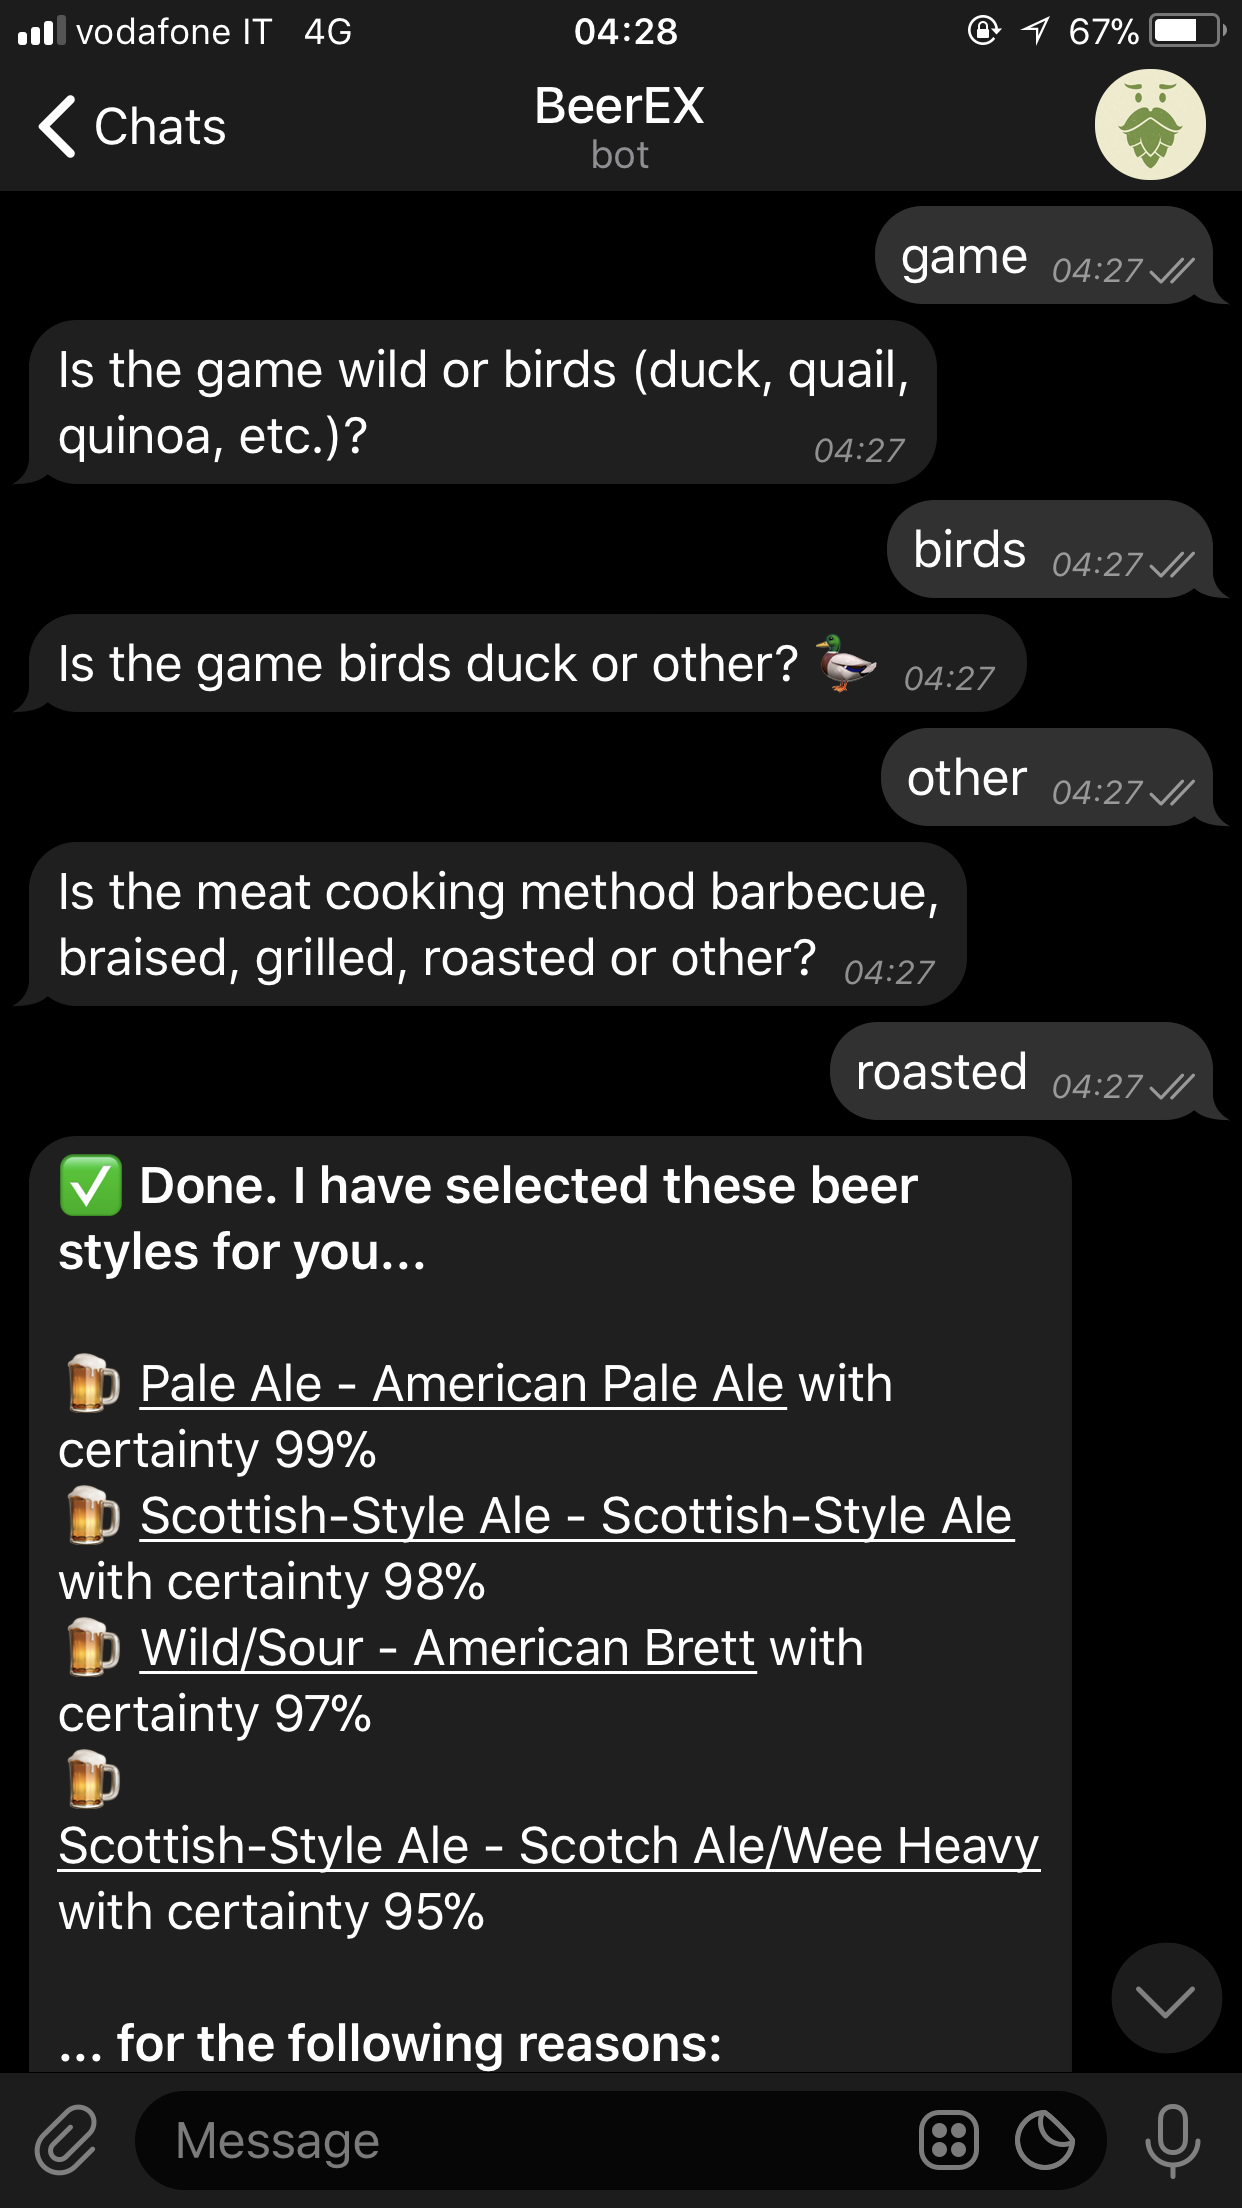
\includegraphics[scale=0.13]{img/bot3.png}\quad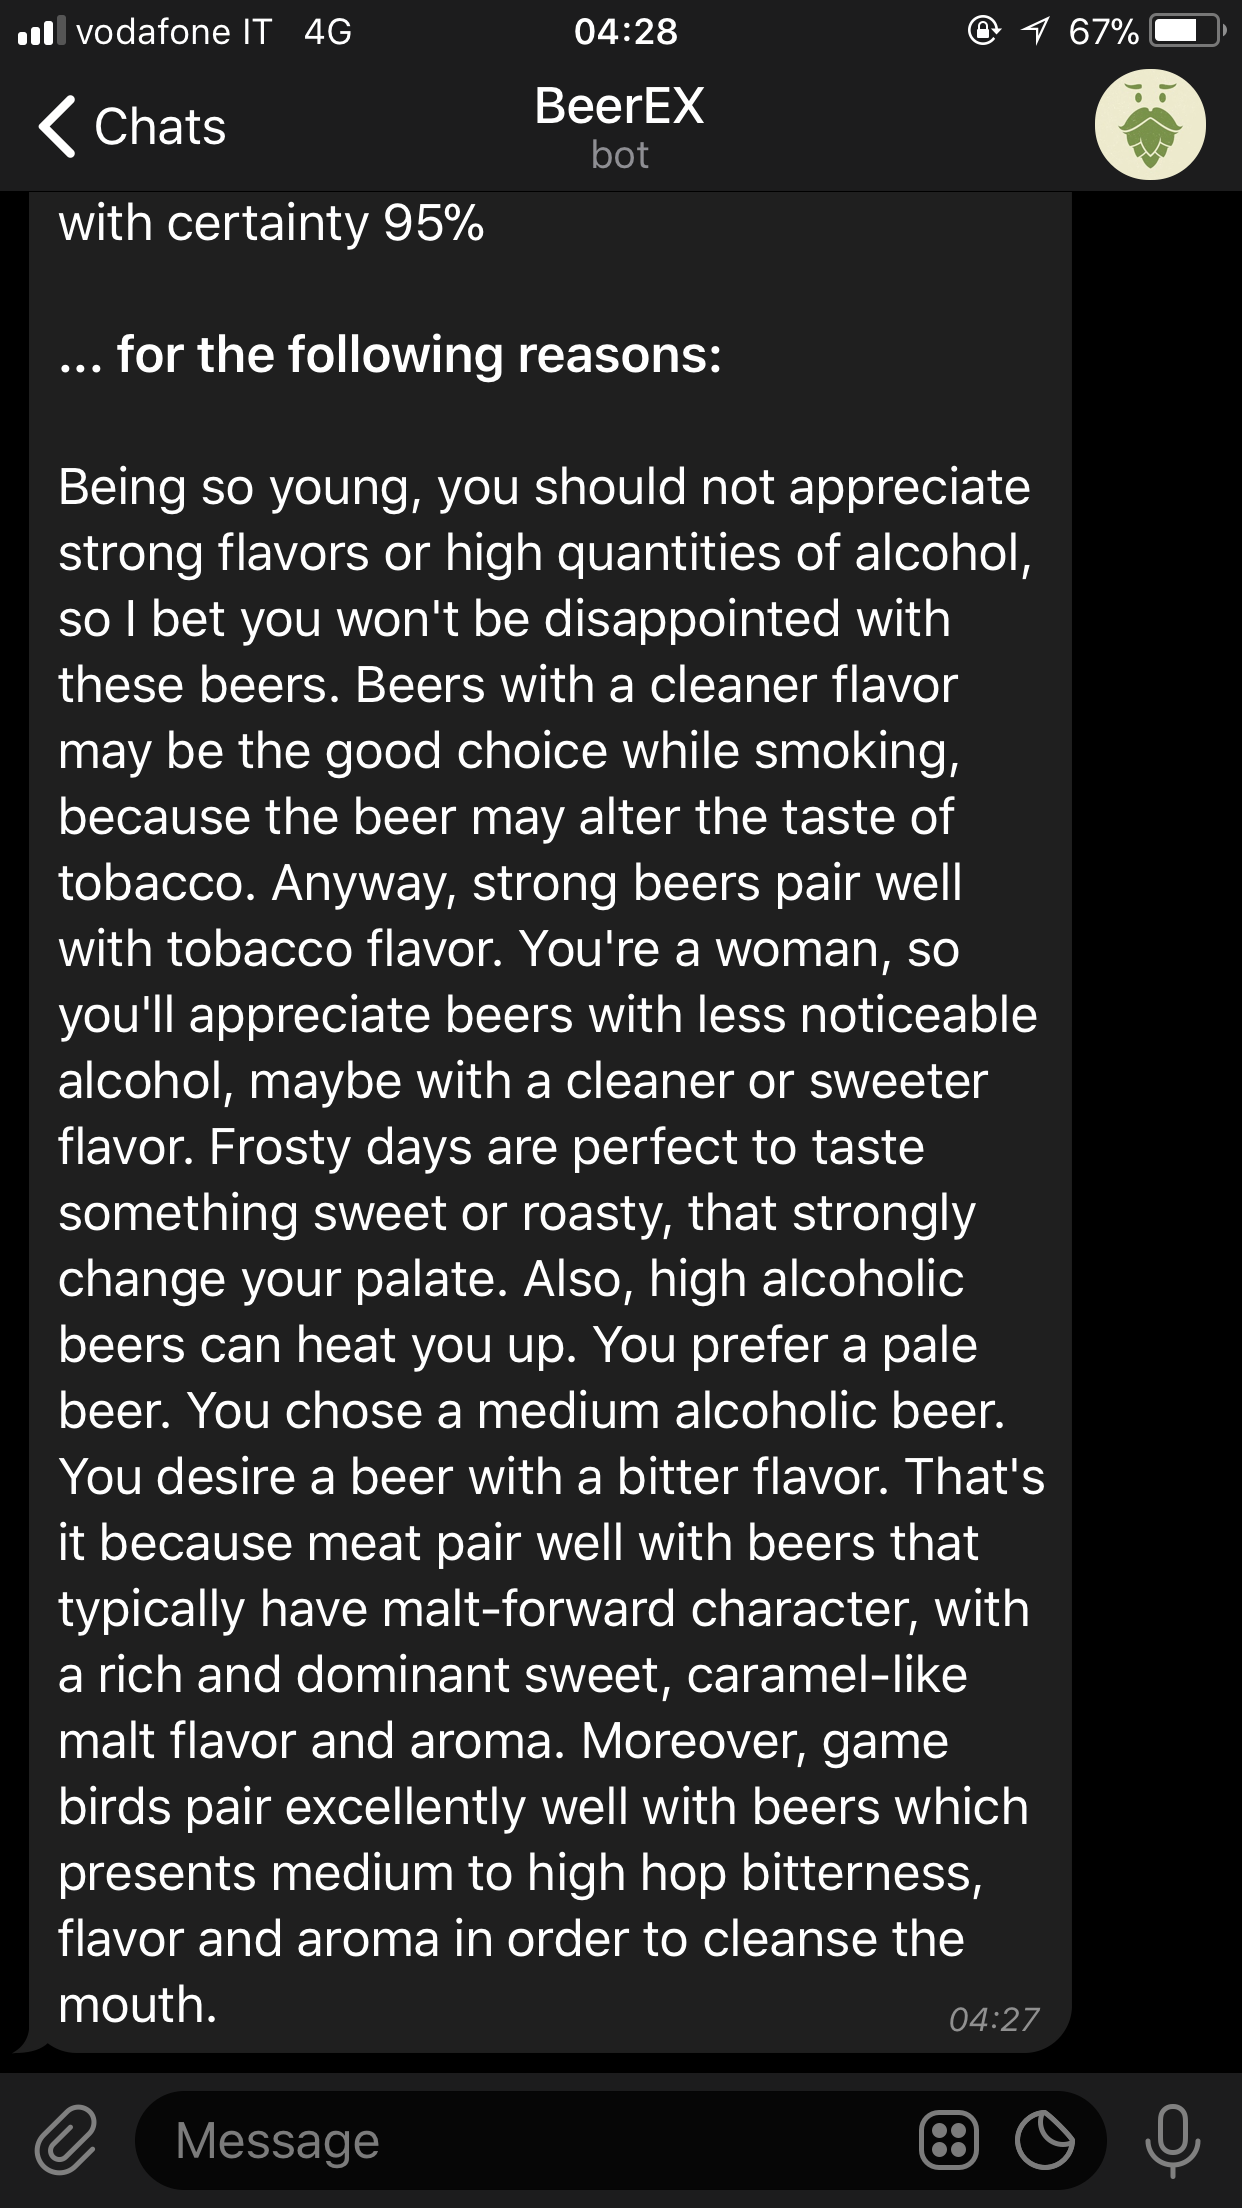
\includegraphics[scale=0.13]{img/bot4.png}
\caption{The chatbot running.}
\end{figure}


\newpage
\bibliographystyle{plain}
\bibliography{biblist}

\end{document}
